
This section shows the results in applying our optimization technique.  The
experimental setup in terms of applications, system software and hardware is
the same as in section~\ref{sec:setup}.  For our evaluation we focus on an 80W
power budget (see \emph{Configurations} in Section \ref{sec:setup}). 

\begin{figure*}[p]
	\centering
        \begin{subfigure}{0.7\columnwidth}
        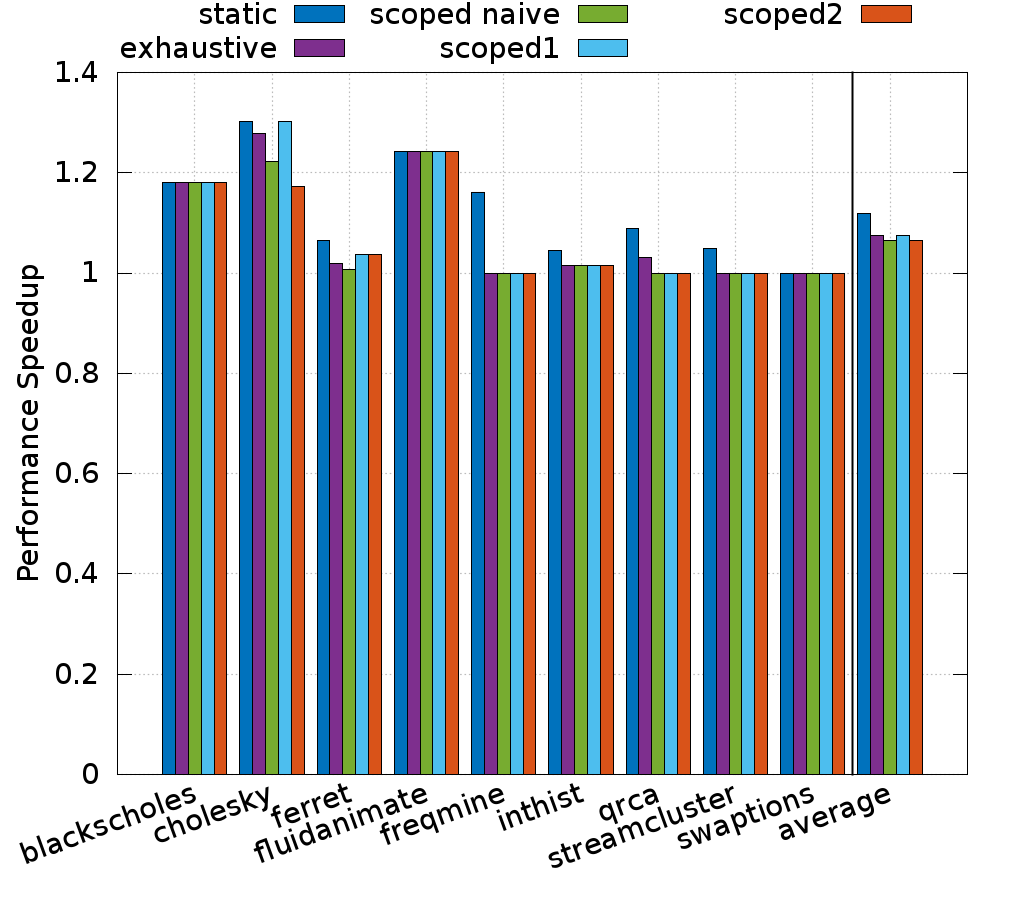
\includegraphics[width=\columnwidth]{power_aware_runtime/figures/dynamic_conf_performance_win1000000}
        \caption{Performance benefits of the selected configurations without accounting for the cost of the search.}
        \label{fig:net_benefit}%
        \end{subfigure}
        \hfill
        \begin{subfigure}{0.7\columnwidth}
        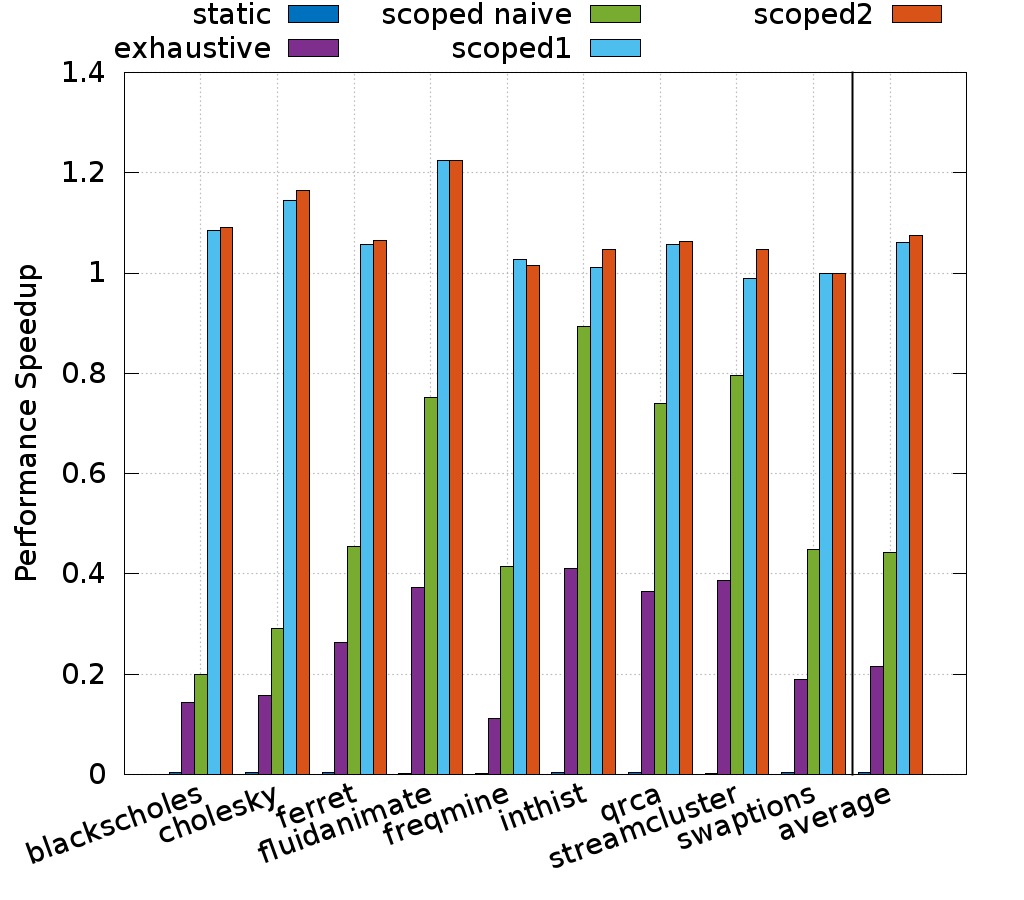
\includegraphics[width=\columnwidth]{power_aware_runtime/figures/dynamic_conf_cost_inv_win1000000}
        \caption{Performance benefits of the selected configurations taking into account the cost of the search.}
        \label{fig:dynamic_analysis_cost}%
        \end{subfigure}
        \caption{Performance benefits using monitoring windows of 1 second under 80 W power limit.}
\end{figure*}


\subsection{Monitoring Window Sensitivity}
\label{sec:window_size_impact}

This first section shows how an optimal window size is obtained by obtaining a detailed
sensitivity study.  This optimal size is leveraged in the following general evaluation of
the search algorithm in terms of its costs and benefits depending on the training set.


Figure~\ref{fig:mon_win_size_impact} shows how window sizes of 0.5, 1, 2 and 5 seconds
influence the effectiveness of the algorithmic search under an 80W power constraint.  The
x-axis represents the considered windows sizes for each application, while the y-axis
shows the speedups obtained over the trivially balanced configuration (40W and 12 active
cores per socket), represented in the figure with red horizontal lines.  The blue
horizontal line represents the speedups achieved by the optimal configuration found using
the multi-execution analysis presented in Section~\ref{sec:static_analysis} .  Purple and
green lines show results considering the exhaustive and scoped naive search spaces
described in section~\ref{sec:searchspaces}, while the blue and the orange lines represent
the scoped1 and scoped2 search spaces.  These results do not consider the cost of the
search algorithm, just the benefit of the optimal configurations found when using
different windows sizes and training sets.

Results shown in Figure~\ref{fig:mon_win_size_impact} clearly show that a windows size of
0.5 seconds on average does not provide  any gain when using the scoped naive training set
and only marginal gains when using the exhaustive search.  Indeed, the exhaustive and
scope naive searches bring significant performance degradations in cases like
\texttt{ferret} and \texttt{qrca} and fail in providing a configuration that delivers the
potential performance gains in case of \texttt{fluidanimate}.  When considering the
scoped1 and scoped2 training sets, 0.5 seconds window sizes do not provide significant
benefits in case of \texttt{ferret} and \texttt{qrca}.  On average, 0.5 seconds large
windows provide average speedups of 1.02x, 0.98x, 1.07x and 1.06x when exhaustive, naive
scope, scope1 and scope2 training sets are used.   

Increasing the windows size from 0.5 to 1 second improves the quality of the
configurations selected. 

Indeed, it provides speedups of 1.27x, 1.22x, 1.30x and 1.17x for \texttt{cholesky} or
1.24x, 1.24x, 1.24x and 1.24x for \texttt{fluidanimate} when exhaustive, trivial scoped,
scoped1 and scoped1 searches are used, respectively.  On average, the 1 second window size
provides benefits of 1.08x when exhaustive search is used and 1.07x when the trivial scope
set is considered, 1.08x when the scope1 is considered and 1.07x for the scope2.  As a
reference, when running a whole execution per each configuration we get optimum power and
active core distribution that bring average speedups of 1.12x.  Increasing the windows
sizes to 2 and 5 seconds does not significantly improve the results quality although they
asymptotically get closer to the ones obtained using the multi-execution analysis.  In
conclusion, the 1 second window size is the optimal one since it provides similar benefits
for all the considered training sets as the 2 and 5 second window sizes under a lower
cost.

The search algorithm works very well for applications with regular computations separated
by barriers (\texttt{blackscholes}, \texttt{fluidanimate} or \texttt{cholesky}) since each
monitoring window can capture different iterations of the same behavior.  In case of
\texttt{ferret} or \texttt{qrca} the scarcity of barriers or synchronization points
reduces the potential gains of our techniques.  When computations are more irregular, it
is more challenging to have consistent monitoring windows, which reduces the effectiveness
of our scheme.  In the particular case of \texttt{freqmine} the task type that accounts
for more than 90\% of the execution is input dependent and actually a single instance of
this task type can take up to half of the total execution time.  As a result the vast
majority of the considered configurations are dismissed since their corresponding
monitoring windows either mismatch or fail to capture any information.

\begin{figure*}[p]
				\centering
        \begin{subfigure}{0.7\columnwidth}
        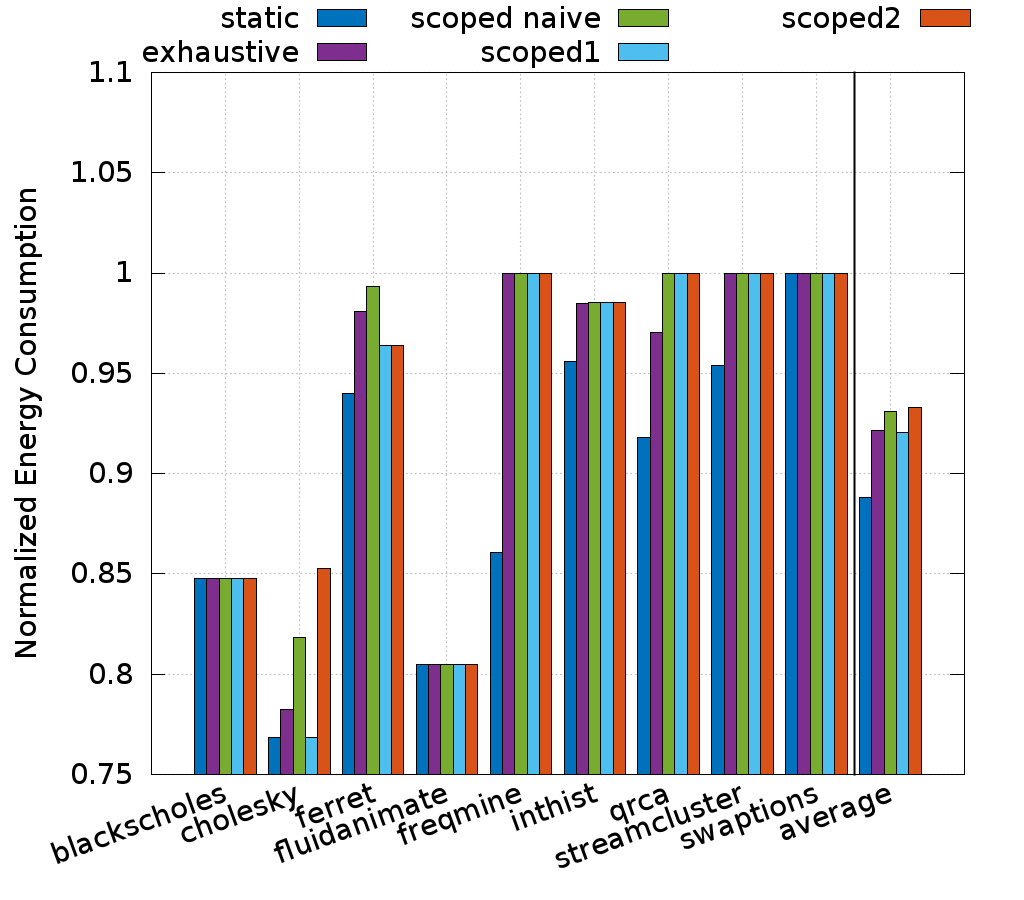
\includegraphics[width=\columnwidth]{power_aware_runtime/figures/dynamic_conf_energy_consumption_win1000000}
        \caption{Energy reductions of the selected configurations without accounting for the cost of the search.}
	\label{fig:dynamic_analysis_energy_consumption_no_cost}
        \end{subfigure}
	\hfill
        \begin{subfigure}{0.7\columnwidth}
        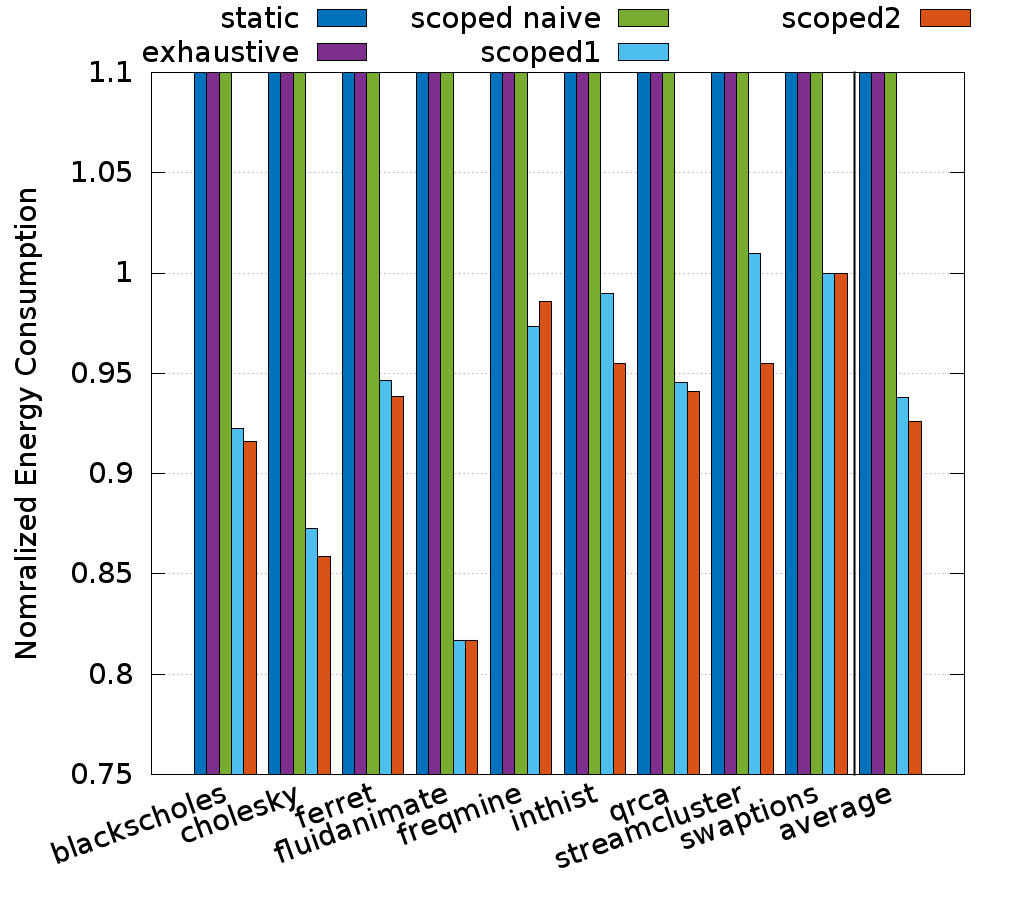
\includegraphics[width=\columnwidth]{power_aware_runtime/figures/dynamic_conf_energy_consumption_w_cost_win1000000}
        \caption{Energy reductions of the selected configurations taking into account the cost of the search.}
        \label{fig:dynamic_analysis_energy_consumption_w_cost}
        \end{subfigure}
        \caption{Energy consumption reduction using 1 second monitoring windows under a 80 W power bound.}
        \label{fig:dynamic_analysis_energy_consumption}
\end{figure*}

\subsection{Performance Improvements of the Selected Configurations}
In Figure~\ref{fig:net_benefit} we show in detail the performance benefits provided by the
optimal configurations found by each one of the four training sets considering a 80W power
bound and 1 second long monitoring windows.  The results are expressed in terms of speedup
with respect to the execution time when using the naive even distribution (40W:40W and
12-12 active cores).  The static technique consists of entirely running the applications
for each one of the 180 configurations defined in Section~\ref{sec:setup}.  The results of
the static technique have already been presented in Section~\ref{sec:static_evaluation}.
This technique, while prohibitively expensive in practice as it requires 180 runs per
application, always finds the best possible configuration and hence provides an upper
bound of the speedup possible. We represent its results in Figure~\ref{fig:net_benefit}.

In case of \texttt{blackscholes} and \texttt{fluidanimate}, all the training sets
(exhaustive, naive scoped, scoped 1 and scoped 2) find configurations that provide the
same speedup as the static technique, 1.17x and 1.24x respectively.  In case of
\texttt{cholesky}, the exhaustive and scoped 1 training sets allow the system to find
configurations that provide speedups very close to 1.3x, the best possible one.  The naive
scope and scoped 2 techniques provide speedups close to 1.2x.  Although these benefits are
significant, they are far from the ones achieved by the other techniques.  The reason is
that the \texttt{cholesky} application benefits a lot from unbalanced distributions
(Table~\ref{table:optimal_configuration}), which are neither considered by the naive scope
nor by the scoped 2 training sets.  In case of \texttt{freqmine}, although the optimal
identified configuration by the static analysis does provide significant benefits, the 4
training sets considered by the searching algorithm fail in finding this optimal
configuration, since tasks are input dependent and can take up to half of the execution
time, as a result most windows fail to capture task throughput since not tasks finish
execution.  In case of \texttt{ferret}, \texttt{inthist}, \texttt{qrca} and
\texttt{swaptions}, the potential benefits of power and active cores balancing are very
limited, since these applications do not have a significant number of barrier
synchronizations.  As we have explained in Section~\ref{sec:nobarriers}, when the overall
number of barriers is not significant, classical load balancing mechanisms are enough to
maximize performance under low power scenarios.

On average, all  training sets provide benefits of around 1.07x, while the static
technique provides an average speedup of 1.11x.  The training costs of the five approaches
are not considered in Figure~\ref{fig:net_benefit}.

\subsection{Performance Improvements Taking into Account Analysis Costs}
\label{sec:costs}
All considered techniques require an analysis to find a power/active cores balance that
optimally improves the trivially balanced distribution.  This analysis starts once the
execution of the parallel code begins and finishes when all the considered configurations
have been tested.  If a single application run is not sufficent to test all the
configurations of the training set, the application is run again and again until the
training is complete.

Figure~\ref{fig:dynamic_analysis_cost} shows the speedups achieved by all considered
techniques including the training phase costs.  In case of the static analysis it is
required to run the application multiple times, one per each of the 180 different
power/active cores distributions.  Consequently, the overall speedup is 0.003x, much
smaller than 1x.  The exhaustive training set considered 180 distributions and checks
their performance over monitoring windows that are 1 second long.  Therefore, more than
one run is required to test all the configurations for those applications with execution
times smaller than 180 seconds.  Since this is the case of all the considered parallel
codes, the average speedup achieved by the exhaustive training set is 0.21x.  Similarly,
the trivial scoped training set obtains a speedup of 0.44x.  These three techniques do not
improve the trivial approach which consists in just evenly distributing the total
available 80W power budget and using all the cores available in the 2-socket NUMA node.

The scoped 1 and 2 training sets consider much fewer configurations than all  previously
mention approaches and, therefore, their training costs are significantly smaller.
Indeed, they are able to test all configurations for 1 second, select the best one and
then run the rest of the application using this optimal configuration.  Of course, the
cost of the training phase can reduce the overall benefits of the optimal configuration,
as it is the case of \texttt{blackscholes}, where the benefits of the scoped 1 and 2
training sets are reduced from 1.17x to 1.08x and 1.09x respectively.  \texttt{Cholesky}
and \texttt{fluidanimate} have larger execution times than \texttt{blackscholes}, which
allows them to compensate the cost of the training phase when scoped 1 and 2 training sets
are considered and to keep almost the same performance gains as if the training costs were
not considered (1.15x and 1.22x, respectively).

Finally, Figure~\ref{fig:dynamic_analysis_cost} reports marginal performance benefits for
some applications for which the search algorithm does not find any distribution
significantly better than the trivial.  For example, in case of \texttt{qrca} there are
speedups of exactly 1x in Figure~\ref{fig:net_benefit}, but of 1.05x and 1.06x for scoped1
and scoped2 in Figure\ref{fig:dynamic_analysis_cost}.  The explanation of this behavior is
that, although the search algorithm fails to find any configuration that is significantly
better than the evenly distributed, there are indeed many configurations that perform
slightly faster than the even one, which accelerate the execution as they are used during
the training phase.

Overall, the static technique and the exhaustive and trivial scope training sets produce
an overall performance slowdown, which makes these approaches useless in practice.  On the
other hand, the scoped 1 and 2 training sets provide important performance benefits even
when the search phase is taken into consideration, which makes these approaches very
useful to maximize performance in power constrained scenarios.

\subsection{Energy Consumption Reductions}
\label{sec:energy}
Figure~\ref{fig:dynamic_analysis_energy_consumption_no_cost} shows the energy consumption
reductions achieved when using configurations found by the five different techniques if
training costs are not considered.  The baseline is the energy spent by the trivially
balanced configuration (12 active cores and a maximum of 40W per socket) and all results
are normalized to this baseline.  The configurations selected by the static analysis
provide energy reductions of 11\% with respect to the even distribution since the
normalized energy gets reduced from 1 to 0.89.  The reductions provided by the search
algorithm are between 7\% and 8\%, depending on the training set.

Once the cost of the exploration phase is considered, the energy consumed by the static
analysis, the exhaustive and the scope naive training sets are 295, 3.7 and 1.8 times
larger than the energy consumed by a single run with the even configuration.  In
Figure~\ref{fig:dynamic_analysis_energy_consumption_w_cost} we just represent normalized
energy consumptions below 1.1 for readability purposes.  As observed before, the scoped 1
and 2 training sets are able to compensate the cost of the training set and deliver
improvements over the even configurations.  The energy consumption reductions are 0.94 and
0.93 for the scoped 1 and 2 training sets respectively.
